%% Master thesis on Adaptive learning of programming.
\documentclass[
    %printed,
    digital,
    color,
    11pt,
    nocover,
    table,  % coloured tables; (to disable: notable)
    nolof,  % hide List of Figures
    nolot,  % hide List of Tables
    microtype,
    %final,
]{fithesis3}
%% Locales.
\usepackage[resetfonts]{cmap}
\usepackage[T1]{fontenc}
\usepackage[
  main=english,
  english, czech
]{babel}
%% Metadata.
\thesissetup{
    date          = \the\year/\the\month/\the\day,
    university    = mu,
    faculty       = fi,
    type          = mgr,
    author        = Tomáš Effenberger,
    gender        = m,
    advisor       = {doc. Mgr. Radek Pelánek, Ph.D},
    title         = {Adaptive System for Learning Programming},
    TeXtitle      = {Adaptive System for Learning Programming},
    keywords      = {adaptive learning, student modeling, learning programming},
}
%% Bibliography.
\usepackage[backend=biber, 		% use biber as backend instead of BiBTeX
	bibstyle=ieee-alphabetic, 	% bibliography style: IEEE with alphabetic citations
	citestyle=alphabetic, 		% citation style
	url=true, 			        % display urls in bibliography
	hyperref=auto,			    % detect hyperref and create links
]{biblatex}
\addbibresource{thesis.bib}
%% Abstract.
\thesislong{abstract}{%
TBA: abstract
}
%% Thanks.
\thesislong{thanks}{%
TBA: thanks, TBA: mention RH and MU projects
}
%% Index.
\usepackage{makeidx}      %% The `makeidx` package contains
\makeindex                %% helper commands for index typesetting.
%% Compact lists.
\usepackage{paralist}
\usepackage{enumitem}
\setitemize{noitemsep,topsep=3pt,parsep=3pt,partopsep=3pt}
%% Mathematics
\usepackage{amsmath}
\usepackage{amsthm}
\usepackage{amsfonts}
%% Graphics
\usepackage{tikz}
%% URLs.
\usepackage{url}
\usepackage{hyperref}
\begin{document}

\chapter{Introduction}
\label{chap:introduction}

Artificial intelligence is a powerful tool for tackling difficult problems,
from playing chess to driving autonomous cars.
This thesis explores how we can use artificial intelligence to optimize
learning of introductory programming.
%This thesis explores how can be artificial intelligence used to optimize
%learning of introductory programming.

Adaptive learning systems have been already successfully used in many domains
\cite{alg.evaluation-geography} (+CITE).
However, the most popular introductory programming tutorials
(Hour of Code) still use a fixed sequence of tasks for everybody,
leading to a suboptimal experience.
Aritificial intelligence can be used to personalize the sequence of tasks
for each student.
By giving students tasks of optimal difficulty, neither too easy, nor too
difficult, we help them to achieve complete immersion into the problem solving
activity, which is known as a \emph{state of flow} \cite{flow}
(figure \ref{fig:flow}).
The state of flow is essential for the optimal learning experience
\cite{adaptive-practice}.

\begin{figure}[htb]
  \centering
  \begin{tikzpicture}[font=\sffamily,xscale=5, yscale=5]
  \large
  %\draw [lightgray, fill=gray] (0,0) -- (0.1,0) -- (1,0.8) -- (0.8,1) -- (0,0.1) -- (0,0);
  \draw (0.1,0) -- (1,0.8);
  \draw (0,0.1) -- (0.8,1);
  \draw [thick, <->] (0,1) node [left] {$challenge$} -- (0,0) -- (1,0) node [below right] {$skill$};
  \node at (0.27,0.82) {frustration};
  \node at (0.6,0.6) {flow};
  \node at (0.7,0.2) {boredom};
  \end{tikzpicture}
  \caption{Relationship between challenge and skill.}
  \label{fig:flow}
\end{figure}

%TODO: related areas
%- introductory programming learning
%- adaptive learning / intelligent tutoring systems
%- recommendation systems (with performance instead of ratings)
%- HCI, (software learnability)
%- games design \cite{book-of-lenses}

How can be domain and students of introductory programming modelled?
Which algorithms to use for task recommendation and mastery learning?
How to evaluate components of the adaptive learning system?
%How to evaluate if the adaptivity of the system helps to improve learning and engagement?
% TODO: Make sure these questions are answered in the text (or remove them).
To answer these questions, we not only look at the existing systems
and research, but we also develop our own adaptive learning system for
introductory programming\footnote{Available at \url{en.robomise.cz}}
(figure \ref{fig:robomission-task1}).
Devopment of this system helps us to better understand related challenges
and enable us to collect data for analyses we need to support or reject our hypotheses.
% TODO: And are there such hypotheses in the thesis?

% TODO: English screenshot.
\imgW[0.9]{robomission-task1}%
  {RoboMission -- application for learning programming.}

We first look at how the introductory programming is currently taught
(chapter \ref{chap:learning-programming}),
and explore relevant techniques of adaptive learning (chapter \ref{chap:adaptive-learning}).
%We focus on models of domain and student for introductory programming,
%algorithms for task recommendation and mastery learning,
%and evaluation of the system and its components.
Then, we describe a new game designed for learning introductory programming
(chapter \ref{chap:design-of-game}),
adpativity of our system (chapter \ref{chap:design-of-adaptivity}),
and its implementation (chapter \ref{chap:implementation-of-robomission}).
We conclude the thesis with analyses of collected data
(chapter \ref{chap:analysis}).

\chapter{Learning Programming}
\label{chap:learning-programming}

\itquote[1mm]{
Learning to write programs stretches your mind, and helps you think better, creates a way of thinking about things that I think is helpful in all domains.
}{B. Gates}

% TODO: Rephrase (avoid "this chapter describes")
This chapter describes the current state of the art of teaching programming, both from the view of successful learning systems and from the view of the research on learning programming.

\section{Existing Systems for Learning Programming}
\label{sec:existing-systems}

% TODO: Rephrase (avoid "presented"?)
There are many systems for learning programming and they differ from each other
in several significant aspects, which are presented in \cref{tbl:existing-systems-categorization}.

\begin{table}[htb]
\centering
\begin{tabular}{l l}
\toprule
Aspect & Examples \\
\midrule
Tangibility & computer applications, physical toys \\
%Target group & primary school, high school students \\
  % Target group interacts with prerequisites
Prerequisites & reading, typing, mathematics \\
Content & loops, variables, functions \\
Form & tasks, videos, texts \\ % worked-out examples,
Tasks & robot on grid, drawing with turtle \\
% Playing-learning ratio & mostly playing, mostly learning \\
Programming language & block-based, textual \\
Adaptivity & task recommendation, mastery learning \\
%Price & free, paid
\bottomrule
\end{tabular}
\caption{Differentiating aspects of systems for learning programming.}
\label{tbl:existing-systems-categorization}
\end{table}


% TODO: Consider to add an interesting fact/observation after the table,
% (or possibly citation pointing to some more broad overviews);
% (linking the table to the rest of the section)
% and consider to move the following "meta-information" to the chapter intro.
The rest of this section briefly describes the most notable existing systems,
focusing on their features that improve learning or engagement.
Section \ref{sec:strategies-for-easier-learning} then extrapolates useful
strategies for teaching programming.


\subsection{LightBot}
\label{sec:lightbot}
LightBot%
\footnote{Available at \url{http://lightbot.com/}.}
is a mobile and web application offering a fixed sequence of tasks solved by
a block-based programming language
(\cref{fig:lightbot}).
%(figure \ref{fig:lightbot-instruction}).
Students create short programs to control a robot in a grid world.
The robot can not only walk and turn left or right, but also jump and turn on lights.
Having five different basic actions is useful for diversity of elementary tasks.
The system covers sequences of commands, procedures, simple loops via tail-recursion,
and conditional commands.

%\subsection{Robozzle}
%\label{sec:robozzle}
%With a robot on a grid and block-based programming, Robozzle%
%  \footnote{Available at \url{http://www.robozzle.com/}.}
%  is similar to LightBot;
%however, it adds a new feature: colored fields.
%Colors can be used in conditional commands,
%  which allows for hundreds of diverse tasks,
%  including difficult tasks with sophisticated recursion.
%Robozzle also allows users to create their own tasks,
%  which can be tried and rated by other learners.
%
%\imgW[0.8]{robozzle}{Robozzle.}


\subsection{Problem Solving Tutor}
\label{sec:problem-solving-tutor}
Problem Solving Tutor%
\footnote{Available at \url{tutor.fi.muni.cz}.}
includes a few problem sets for practicing programming,
such as Interactive Python, Karel the Robot, or Robotanist
% TODO: more precise description of the tasks instead of e.g. "Inter. Python",
% see the reffed paper for inspiration.
\cite{proso}.
Robotanist (\cref{fig:robotanist}) is similar to LightBot,
with an addition of colored fields.
Colors can be used in conditional commands, which allows for diverse tasks,
including difficult problems with complex recursion.  After
each solved task, Problem Solving Tutor shows a recommendation for two next
tasks %(one easier, on more difficult),
with predicted solving times.
Showing predicted time % to the user
serves as a motivational element, posing
a suitable challenge to overcome oneself
\cite{pelanek-student-modeling-times}.

%\imgW[0.6]{lightbot}{LightBot.}
%\imgW{lightbot-instruction}{LightBot provides clear and simple interactive instructions.}
%\imgW[0.6]{robotanist}{Robotanist in Problem Solving Tutor, Detour task.}


\begin{figure}[htb]
\centering
\begin{subfigure}[t]{0.5\textwidth}
\centering
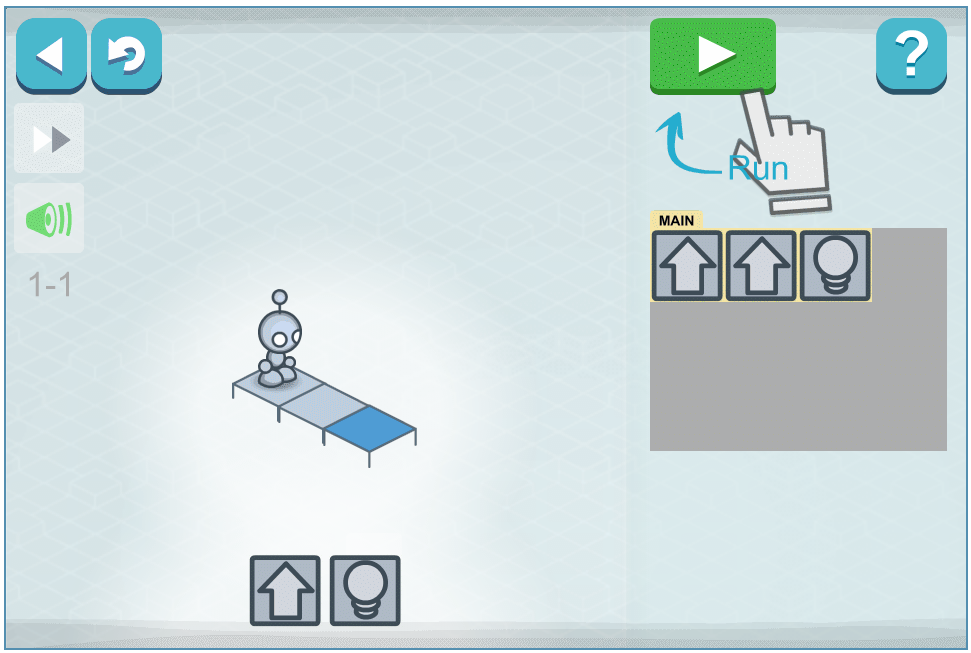
\includegraphics[height=4cm]{img/lightbot-instruction}
\caption{LightBot}
\label{fig:lightbot}
\end{subfigure}%
\begin{subfigure}[t]{0.5\textwidth}
\centering
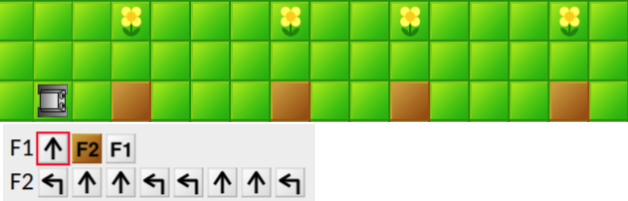
\includegraphics[height=4cm]{img/robotanist}
\caption{Robotanist}
\label{fig:robotanist}
\end{subfigure}
\caption{LightBot and Robotanist provide square grids for commands.}
\label{fig:lightbot-robotanist}
\end{figure}



\subsection{Blockly Games}
\label{sec:blockly-games}
Blockly is a popular block-based programming interface.
In contrast to the blocks in LightBot,
Blockly blocks can be assembled in nested control structures
(\cref{fig:blockly-games}).
Blockly Games%
\footnote{Available at \url{https://blockly-games.appspot.com/}.}
% TODO: Replace by figure using nested control structures
% and move the fre to the end of previous sentence.
%(figure \ref{fig:blockly-instruction})
%demonstrate Blockly usage. The webpage ...
consist of several problem sets with Blockly, ordered by increasing difficulty.
For example, in the first level, students learn how to compose blocks together
as a puzzle, and in the second level they learn loops and conditions by solving
tasks in a maze. Final level serves as a transition from block-based
programming to textual programming in JavaScript.
Each level consists of 5-10 tasks, again ordered by increasing difficulty. %, with no personalization.
The fixed order enables to build on the program from the previous task,
thus gradually leading to more complex programs,
resulting for example in sophisticated images in turtle graphics.
Blockly Games includes non-ignorable interactive instructions,
which require to take a described action before they disappear
\cite{blockly-10-things}.

%\imgW[0.7]{blockly-instruction}%
%  {Blockly Games includes non-ignorable interactive instructions, %
%  which require to take a described action before they disappear.}

\subsection{Hour of Code}
\label{sec:hoc}
Hour of Code%
\footnote{Available at \url{https://hourofcode.com}.}
%(figure \ref{fig:hour-of-code-sw})
provides many one-hour tutorials, each containing about 15 tasks in fixed order,
using Blockly-based language
(\cref{fig:hoc}).
These tutorials focus on motivation, using themes from popular movies and
games, and providing videos with famous people explaining programming concepts.
The tutorials use high-level theme-specific blocks, such as ``set droid to a
random speed``, and they are restricted to only one or two programming
concepts, e.g. sequences of commands and events.
In some tasks, the built program is not a direct solution for a robot,
but rather a game, in which the code specifies actions triggered on events.
% TODO: There is some space to include more info about HoC.

%\imgW[0.7]{hour-of-code-sw}{Hour of Code, Star Wars tutorial.}


\begin{figure}[htb]
\centering
\begin{subfigure}[t]{0.43\textwidth}
\centering
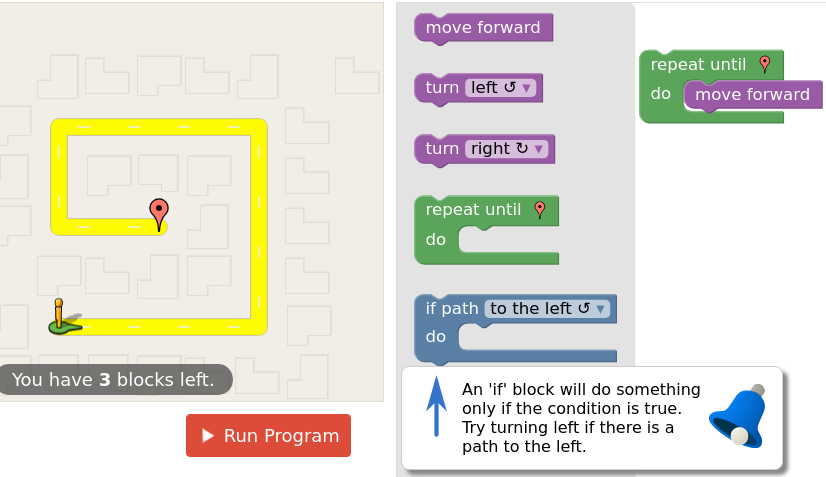
\includegraphics[height=33mm]{img/blockly-nested}
\caption{Blockly Games (Maze level)}
\label{fig:blockly-games}
\end{subfigure}%
~
\begin{subfigure}[t]{0.57\textwidth}
\centering
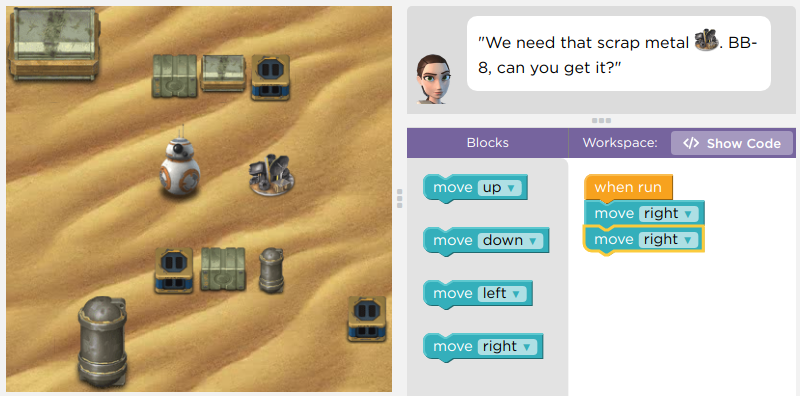
\includegraphics[height=33mm]{img/hour-of-code-sw}
\caption{Hour of Code (Star Wars theme)}
\label{fig:hoc}
\end{subfigure}
\caption{Two programming games using nested blocks.}
\label{fig:blockly-hoc}
\end{figure}





\subsection{Human Resource Machine}
\label{sec:human-resource-machine}
Human Resource Machine%
\footnote{\url{http://tomorrowcorporation.com/human-resource-machine-hour-of-code-edition}}
%\footnote{Free Hour of Code edition available at \url{http://tomorrowcorporation.com/human-resource-machine-hour-of-code-edition}.}
is an example of an offline computer game for learning programming.
%Although it is presented as a game,
%the player spends nearly all the time solving tasks similar to those in the previously mentioned learning systems.
% Removal candidate (1 sentence):
The sequence of tasks is non-personalized and nearly linear,
with a few short side branches.
Similarly to the systems above, it also uses block-based programming,
but now in a different domain:
it offers low-level programming commands, such as
input, output, move-from, move-to, add, or jump
%(figure \ref{fig:human-resource-machine}).
(\cref{fig:hrm}).
% input, output, move-to, move-from, add, sub, jump, jump-nonzero, jump-negative.
The programming environment includes a debugger,
providing a possibility to step through the program.
All concepts are explained when they first appear in the game,
and programming blocks can
be explained again simply by dragging the block onto a dedicated field with a question
mark.

%\imgWithFootnote[0.7]{human-resource-machine}{Human Resource Machine}%
%{Source: \url{https://tomorrowcorporation.com/humanresourcemachine}}
%%{Source: \url{https://tomorrowcorporation.com/humanresourcemachine} (Tommorow Corporation).}

\subsection{Khan Academy}
\label{sec:khan-academy}
Khan Academy has a computer programming curriculum%
\footnote{Available at \url{https://www.khanacademy.org/computing/computer-programming}.}
that uses textual programming in JavaScript with functions for drawing shapes
in absolute coordinates %(figure \ref{fig:khan-academy}).
(\cref{fig:ka}).
In addition to programming tasks, it contains text and video explanations, and
projects. Some videos are in the form of interactive \emph{talk-throughs},
in which the student can fiddle with the explained code at any moment to understand
how it works.

%\imgW[0.8]{khan-academy}%
%  {Parting Clouds programming task on Khan Academy.}


\begin{figure}[htb]
\centering
\begin{subfigure}[t]{0.48\textwidth}
\centering
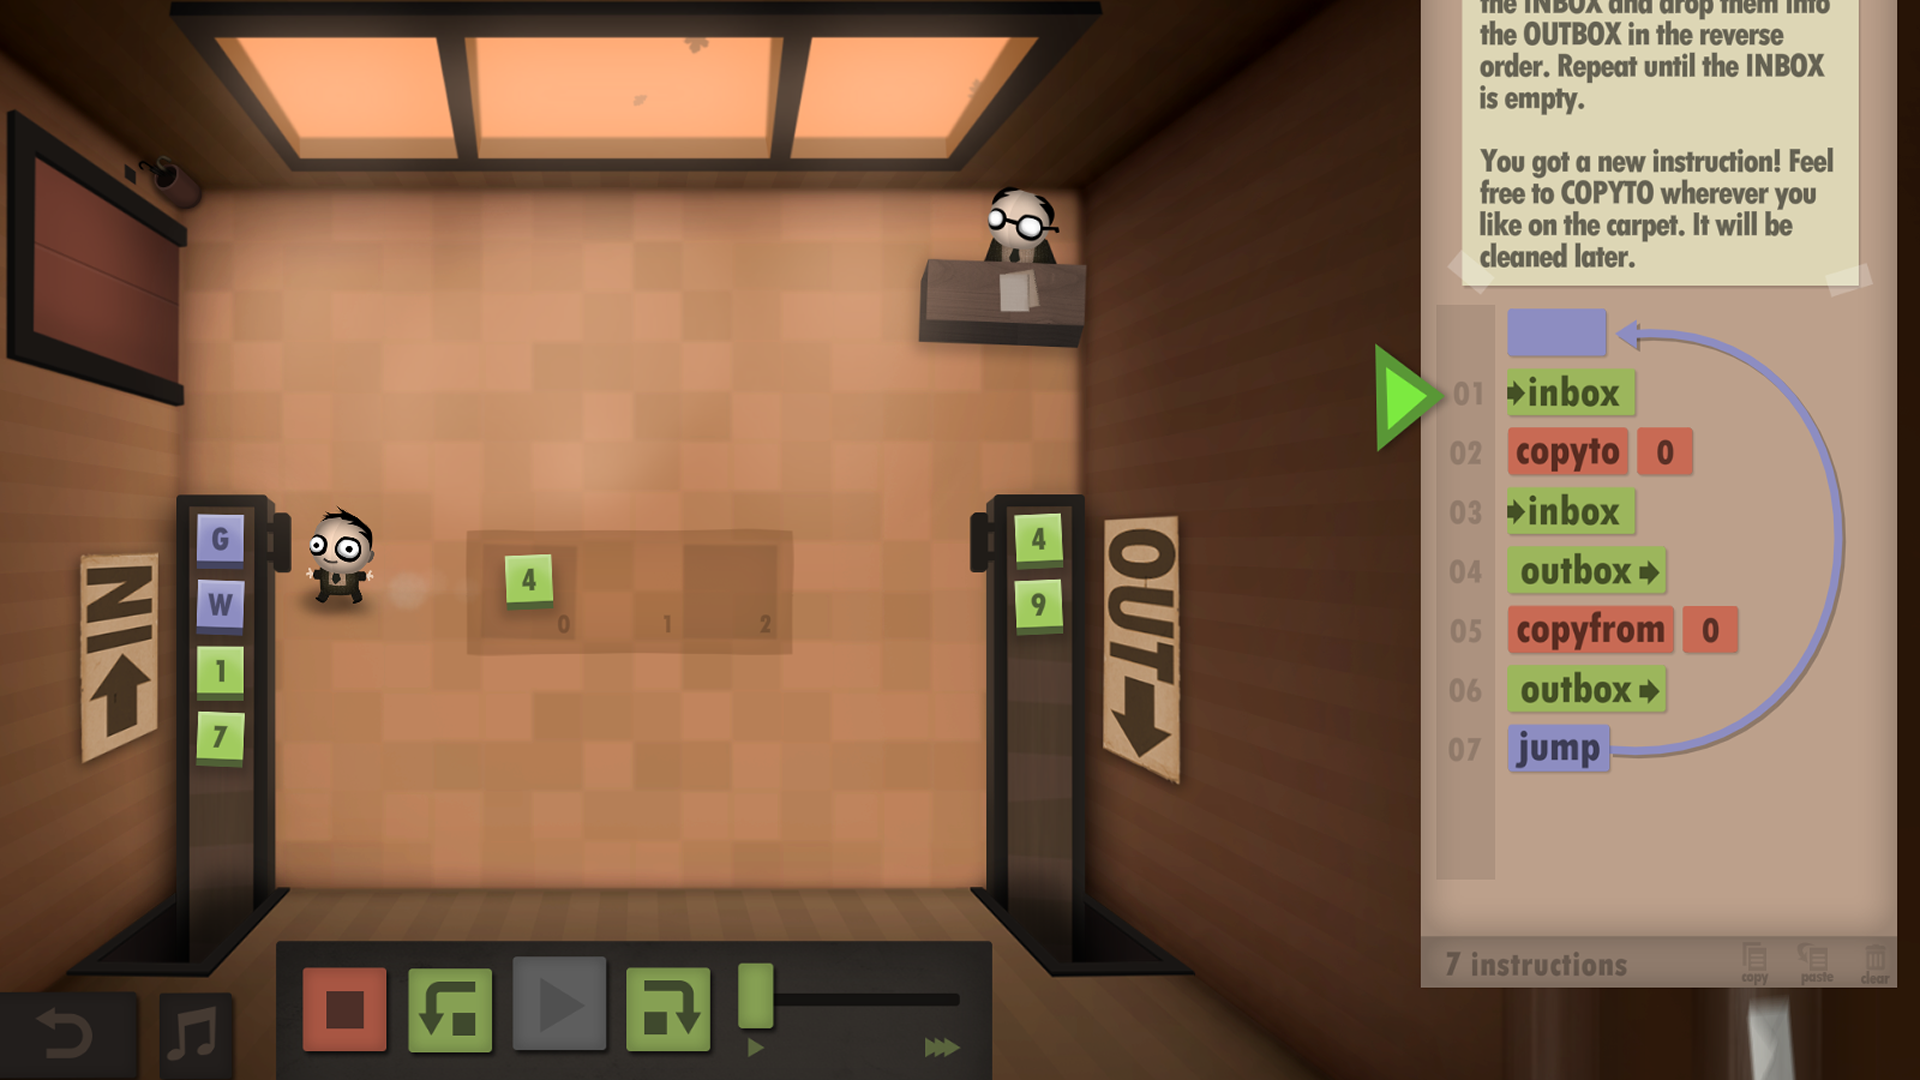
\includegraphics[height=30mm]{img/human-resource-machine}
\caption{Human Resource Machine\protect\footnotemark}
\label{fig:hrm}
\end{subfigure}%
\begin{subfigure}[t]{0.52\textwidth}
\centering
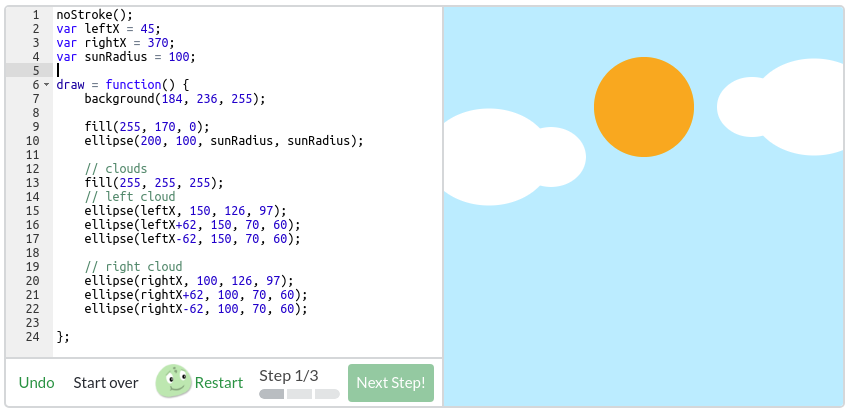
\includegraphics[height=30mm]{img/khan-academy}
\caption{Khan Academy}
\label{fig:ka}
\end{subfigure}
\caption{Tasks using Assembly-based and JavaScript-based languages.}
\label{fig:hrm-ka}
\end{figure}
\footnotetext{Source: \url{https://tomorrowcorporation.com/humanresourcemachine}.}






%\subsection{We Can Code}
%\label{sec:umime}
%
%TODO: present UmimeProgramovat -> turtle graphics, mastery learning
%\footnote{Available at \url{https://www.umimeprogramovat.cz/} (Czech only).}


%\subsection{Ozobot}
%\label{sec:ozobot}
%Ozobot%
%\footnote{Product webpage available at \url{http://ozobot.com/}.}
%is a small physical robot
%programmable by either a Blockly-based interface,
%  or even without a computer
%  by drawing lines on a paper and reading them with a color sensor on the robot.
%As it does not require ability to read and write
%  Ozobot is suitable for even very young children.

%\imgWithFootnote[0.8]{ozobot-robot}{Ozobot}%
%{Source: \url{https://www.flickr.com/photos/robpegoraro/19464353039}, Rob Pegoraro.}

%\imgW{ozobot}{%
%  Ozobot simulator (available at \url{http://games.ozoblockly.com}) %
%  is a Blockly-like interface for creating programs for Ozobot %
%  (but the simulater requires the ability to read). %
%  It also includes a few prepared tasks.}


%\subsection{Project Euler}
%\label{sec:project-euler}
%The core of Project Euler%
%\footnote{Available at \url{projecteuler.net}.}
%is a list of several hundreds of programming problems with one correct answer.
%The problems can be solved in any language
%and then checked whether the computed answer is correct.
%The project is not meant to teach elementary programming,
%but rather to hone one’s programming skills;
%more complicated tasks even require some knowledge of algorithms and data structures.
%
%\imgW[0.7]{project-euler-progress}{%
%Project Euler provides several means of motivation: %
%levels (based purely on number of solved tasks), badges %
%(e.g. for solving 10 consecutive problems, 50 prime numbered problems, etc.), %
%comparison with user’s friends, %
%statistics page with several leaderboard (e.g. by country), %
%and a special score based on the performance on the most recently published problems.}


%\subsection{HackerRank}
%\label{sec:hacker-rank}
%
%Online programming contests,
%in which people attempt to solve as many problems as possible
%in limited time frame of a few hours,
%became popular in the last years.
%In addition to organizing such contests regularly,
%HackerRank%
%\footnote{Available at \url{https://www.hackerrank.com/}.}
%also provides many training programming tasks for various topics,
%from introductory programming to machine learning.
%% Solutions are evaluated on a server against a prepared set of test cases with time limits.
%In addition to the classic motivation in the form of points, badges and leaderboards, students are motivated to practice to perform well in the competitions,
%where they can win some prizes and sometimes even job offers.
%HackerRank also helps student to decide on a problem to solve by showing its difficulty according to the author of the task (on a 3-star scale),
%as well as success rate among the past submissions.
%Furthermore, after solving a task,
%a specific recommendation the next task to solve is shown.


%\imgW[0.6]{hackerrank}{HackerRank. %
%Each task specifies input and output format, including some examples. %
%Solution can be written either locally or in the provided online editor.}


\section{Strategies to Support Learning}
%\section{Strategies for Easier Learning}
\label{sec:strategies-for-easier-learning}

Learning programming is difficult,
  because it requires
  to adopt algorithmic thinking,
  understand program execution,
  and remember formal syntax of a programming language;
  all these three skills at once. % at the same time.
To make learning easier,
  the systems presented in the previous section use diverse strategies,
  such as avoiding syntax errors,
  displaying visual output
  and providing hints.
Various other strategies were tried in the past as well;
article \emph{Lowering barriers for Novice Programmers}
  \cite{lowering-barriers}
  provides a detailed overview.


\subsection{Avoiding Syntax Errors}
\label{sec:avoiding-syntax-errors}

A common strategy for avoiding syntax errors is to replace textual programming
with drag-and-drop block-based programming.
There are two basic types of block-based interfaces:
  either with a square grid defining the program shape,
  often one row per function
  (\cref{fig:lightbot-robotanist}),
  or the blocks can be nested and assembled arbitrarily,
  with no limit on maximum program length,
  often one vertical stack per function
  (\cref{fig:blockly-hoc}).
The fixed square grid is simpler to understand and manipulate with,
  but it does not allow for nesting,
  which is a fundamental feature of computer programs.
This restriction is usually overcome by
  combining condition and commands into a single block,
  by using recursion instead of loops,
  and by replacing nested sequences of commands by a new function.

%TODO: the block-based editors are a special case of "structred editors",
%idea: editor only allows edits that transform the code from one syntactically correct
%program to another (basically working on AST level, edit = transforms to another AST)
%(compared to: classical text editors, where the edit can be arbitraty, making the code
%not syntactically correct).

%\subsection{Potential Drawback of Block-based Interfaces}
%\label{sec:potential-drawback-of-block-based-interfaces}
A drawback of using block-based programming
  is that the students need to learn a proper textual programming language in
  the future to be able to implement more complex programs.
Several controlled experiments were performed to test a hypothesis
  that it is still beneficial to start an introductory programming course
  with a block-based programming,
  even when the students will be writing textual code later in the course
  \cite{comparing-blocks-text-price2015, comparing-blocks-text-weintrop2017}.
Results suggest that block-base interfaces indeed lead to increased learning and
motivation; however, the evidence is not fully convincing. For example, in
some of these studies, the programming interfaces differed in more aspects than
just in using blocks instead of text. Furthermore, these studies do not
answer when it is the right moment to switch from block-based to textual
programming.

%\subsection{Transition Strategy}
%\label{sec:transition-strategy}
%Weintrop and Wilensky suggest that the block representation of the code
To make the transition easier, block representation of the code
  should match the underlying programming language
  to which the student is expected to move in the next phase
  \cite{challenges-of-blocks-based-environments}.
However, resemblance to a programming language sometimes
  conflicts with the readability of the blocks for novices.
Instead of making compromises,
  the system can progressively change the available set of blocks in each level,
  making them more and more similar to a textual programming language.
In the last level of Blockly Games, which employ this strategy,
  the text on the blocks matches the generated JavaScript exactly
  \cite{blockly-10-things}.

%TODO:
%- note: "blending block-based and text-based programming approaches (e.g., Pencil Code
%(Bau 2015), Tiled Grace (Homer and Noble 2014), and Greenfoot’s Frame-based editor (Kölling et al.
%2015)"


\subsection{Visual Output}
\label{sec:visual-output}

Learning systems can help students to track program execution
  by providing a clear visual representation of the current state
  and effects performed by the program.
This can be achieved naturally for turtle graphics,
  where the whole state is just a position and orientation of the turtle,
  and effects are the drawn lines.
Similarly, in simple games, such as those described in
  \cref{sec:lightbot,sec:problem-solving-tutor,sec:blockly-games,sec:hoc},
  the grid world visualization contains complete information about the current
  state (\cref{fig:lightbot-robotanist,fig:blockly-hoc}).
For the simplicity of their visual output,
  drawings and grid world games have become prevalent task types
  in the current systems for learning programming.

\subsection{Instructions and Hints}
\label{sec:instructions-and-hints}

Most educational systems include instructions
  to explain new concepts such as loops and conditions.
%However, Neil Fraser explains that students ignore instructions,
However, many students ignore instructions,
  no matter how prominent they are \cite{blockly-10-things}.
A solution to this problem are actionable non-ignorable instructions,
  which cannot be closed manually by the student, and disappear only once the
  student performs the action described in the instruction
  (\cref{fig:blockly-games}).

In addition to the instructions, some systems offer hints, which appear either
  upon a student request, or automatically after a certain time of unsuccessful
  solving. Although it is possible to generate a hint in any state,
  using data of students which have successfully solved the task before
  \cite{generating-hints}, the existing systems use a few manually prepared
  hints, instead of relying on the automatic approaches.

\section{Strategies to Support Motivation}
%\section{Strategies for Motivation}
\label{sec:motivation}
% NOTE: Prev section: learning, this section: engagement.

In addition to strategies for easier learning presented in section
\ref{sec:strategies-for-easier-learning}, it is equally important to create an
engaging environment supporting students’ motivation.
All strategies for supporting motivation are based on fulfilling some human
needs \cite{nvc}. % TODO: cite specific page
\Cref{tbl:motivation-strategies} links needs to common strategies.
% TODO? related: flow, happiness, switch-elephant (prev. section: path)

\begin{table}[htb]
\centering
\begin{tabular}{ll}
\toprule
Needs & Strategies \\
\midrule
Purpose & Emphasizing usefulness of the programming skill. \\ %, confidence
Progress, learning & Skills visualization, points, levels. \\
Effectiveness & Recommending tasks of optimal difficulty. \\ % concentration/flow
Autonomy & Allowing to choose a topic or a task. \\
Recognition & Badges, leaderboards. \\  %Appreciation  % leaderboard vs. scoreboard?
Sharing & Possibility to share programs or achievements. \\
Cooperation & Pair programming. \\
Beauty, harmony & Appealing game world. \\ %, which is nice to look at and fun to play with \\
Fun & Entertaining tasks. \\
Creativity & Open-ended tasks, projects. \\  %, self-expression
% Community?
\bottomrule
\end{tabular}
\caption{Needs and strategies that help to fulfill these needs.}
\label{tbl:motivation-strategies}
\end{table}



\subsection{Appealing Game World}
\label{sec:motivation.game-world}
Ideally, game world should appeal to students --
even without tasks to solve,
  it should be an interesting toy to play with \cite{book-of-lenses}.
That is why all Hour of Code tutorials are based on movies and games
  popular among children, such as Angry Birds, Frozen, or Star Wars
  (\cref{fig:hoc}).
In such environments, it is possible to assign open-ended tasks,
  or even let the students create whatever they want,
  which works well especially for creative students seeking for self-expression.
For example, Khan Academy programming curriculum contains many several
open-ended drawing projects (\cref{fig:ka}).
%\cref{sec:robomission.game-world}

\subsection{Entertaining Tasks}
\label{sec:motivation.tasks}
For many students, giving them specific small problems works better
  than large, loosely defined, open-ended tasks.
By solving small problems quickly,
  they get a feeling of progress and learning.
Another advantage of closed tasks
  is a more straightforward implementation of gamification features and adaptive behavior.

Small closed tasks result in short programs,
  but their behavior should be still interesting. % for the students to be satisfied.
To achieve complex behavior,
  a system can either provide students with macro-commands (e.g. to draw a circle)
  or with a skeleton of complex code, with a few gaps to fill in by students.
However, it is important for the students to feel ownership over the code,
  which is especially a concern with the code skeleton.
Solution implemented in Blockly Games
  is to make a series of tasks in which the students
  build on their program from the previous task
  \cite{blockly-10-things}.

% TODO: some examples in the form of figures + descriptions
% TODO: other important aspects: variability


\subsection{Optimal Challenge}  % OR: "Optimal Difficulty"
\label{sec:motivation.challenge}
For a great learning experience,
  difficulty of the task must match the skill of the student.
If the task it too easy,
  the student is not challenged and gets bored.
If the task is too difficult,
  the student becomes frustrated and desperate.
On the other hand, if the task has appropriate difficulty,
  the student is likely to be challenged and focused
  (\cref{fig:flow}).
The complete immersion into the task the student is solving at the moment is called
  a state of flow \cite{flow},
  or a \emph{zone of proximal development} \cite{zone-of-proximal-development}.
Achieving the state of flow maximizes the learning outcome \cite{adaptive-practice}.
  % and even increases the long-term level of happiness. % TODO: find a source of this claim
\Cref{chap:adaptive-learning} describes techniques for estimating student's skills
and recommending tasks of optimal difficulty.
% for estimating student’s skill and show how to use that estimate for task recommendation and mastery learning.


\subsection{Gamification and Progress Visualization}

Sense of progress and learning can be boosted by visualizations of
progress towards mastery in the current topic, solved tasks, completed problems sets,
or acquired skills.
\Cref{fig:progress-visualization} shows examples of progress bars from various systems.

% TODO: cite relevant research, open learner model
% NOTE: also helps to decide what to practice next, while preserving student's
% autonomy (soft recommendation)

\begin{figure}[htb]
\centering
\begin{subfigure}{.48 \textwidth}
  \centering
  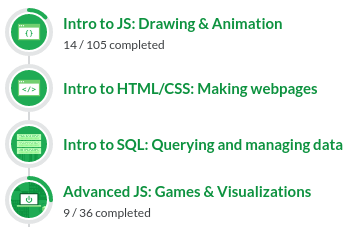
\includegraphics[width=.9\textwidth]{img/ka-skills}
\end{subfigure}
\begin{subfigure}{.48\textwidth}
  \centering
  
\includegraphics[width=.9\textwidth]{img/hour-of-code-progress}
  \bigskip
  \vspace{1mm}
  
\includegraphics[width=.9\textwidth]{img/umime-progressbar}
\end{subfigure}
\caption{%
  Progress bars: Khan Academy topics, Hour of Code tutorial,
  and mastery progress bar in Umíme Programovat (``We Can Code'').}
\label{fig:progress-visualization}
\end{figure}


%\subsection{Gamification}

Although the programming tasks themselves can be considered as a game
(e.g. Human Resource Machine from \cref{sec:human-resource-machine} is
presented purely as a game),
most learning systems add further gamification elements to increase the sense
of progress.
Common gamification elements include points, levels, badges, and leaderboards.

% TODO: figures: Project Euler, KA
% TODO: ref relevant research

\chapter{Adaptive Learning}
\label{chap:adaptive-learning}

% TODO:
% - incorporate other notes from my/thesis gdoc
% - inspiration from relevant articles
% - add references for provided examples (playing chess, autonomous car, ...)

Artificial intelligence proved to be a mighty tool
  for tackling difficult algorithmic tasks,
  from playing chess to driving an autonomous car.
The power of artificial intelligence can be also used
  to develop a personalized adaptive system for learning programming.
Such system should create an optimal learning experience for each student
  by providing them with problems of difficulty matching their skill,
  so that the student stays challenged and interested in solving them.

In the existing systems (\ref{sec:existing-systems}),
  the sequence of tasks is the same for everybody.
As a result, the progress is necessarily too slow for some students,
  who could skip some of the tasks,
  while being too fast for others,
  who could highly benefit from solving many more similar tasks.
Artificial intelligence can be used to personalize
  the sequence of tasks for every student.
By giving the student a suitable task
  -- neither too easy, nor too difficult --
  it can help the student to get into the state of flow
  (\ref{sec:motivation.challenge}).

In addition to choosing the most suitable task for given student,
  artificial intelligence has also other possible uses in learning systems,
  for example automatic hints generation \cite{generating-hints}
  or skills visualization (TBA: ref).
Furthermore, artificial intelligence techniques can be used
  to analyze collected data offline
  and, for example, detect problematic tasks
  or suggest how to group tasks into categories (TBA: ref).

Adaptive learning systems have been already successful in some domains.
For instance, Map Outlines%
  \footnote{Available at \url{https://outlinemaps.org}.},
  developed by Adaptive Learning research group at Masaryk University,
  is an intelligent web application for learning geography.
It has been used by tens of thousands of students
  and online experiments have confirmed
  that the adaptivity of the system helps to improve the learning outcome
  \cite{alg.evaluation-geography}.
In addition to geography, similar adaptive web applications
  for learning anatomy%
  \footnote{Available at \url{https://practiceanatomy.com}.},
  biology%
  \footnote{Available at \url{https://poznavackaprirody.cz} (in Czech only).},
  elementary mathematics%
  \footnote{Available at \url{https://matmat.cz} (in Czech only).},
  and Czech grammar%
  \footnote{Available at \url{https://umimecesky.cz} (in Czech only).},
  were developed by the research group in recent years.

Section \ref{sec:student-modeling} presents how to model students
  in the context of learning programming.
Sections \ref{sec:task-recommendation} and \ref{sec:mastery-learning}
  then describe how to use these models to make a learning system adaptive.
Finally, section \ref{sec:metrics-and-evaluation} discusses how to evaluate
  different models or even whole learning systems.


\section{Student Modeling}
\label{sec:student-modeling}

For the system to be adaptive, models of
  a student skill, task difficulty, and student-task interaction
  need to be designed, implemented and evaluated using collected data.
The purpose of these models is to predict the probability that a given student
  would solve a given task
  and also the time the student would need to complete the task.


\subsection{Data}
\label{sec:student-modeling.data}

To learn model parameters, such as difficulty of individual tasks, some data is needed.
What data is needed and how much differs across models.
Some data about tasks are independent of students;
therefore, they can be obtained in advance,
which can be useful for initial task difficulties estimates.
Three types of task data are distinguished:

\begin{itemize}
  \item task statement (including name and world description),
  \item sample solution (or multiple solutions),
  \item expert labels (e.g. covered concepts).
\end{itemize}

Task statements are always available,
  because they are needed to present tasks to students.
However, obtaining sample solutions and expert labels
  incurs additional costs for a new system.
% TODO: Note that quite often, systems needs sample solutions and some labels
%       for the presentation purposes anyway.
Moreover, they can be noisy and imperfect.
For example, an annotator can forget to include some labels
  or even make a mistake in the sample solution.

Once the task is deployed in the running system,
  rich data can be collected from each interaction between a student and a task:
\begin{itemize}
  \item whether the task was eventually solved,
  \item solving time,
  \item number of clicks, number of code executions,
  \item program snapshots (e.g. after each code change),
  \item rating or labels provided by the student (e.g. perceived difficulty).
\end{itemize}

% TODO: also consider to include hints in the list
% TODO: mention different granularity levels for taking program snapshots (+cite)

\subsection{Item Response Theory}
\label{sec:irt}

The simplest version of item \emph{item response theory} (IRT)
  \cite{irt-visual-guide}
  models each student by a one-dimension skill $s$,
  and each task by a one-dimension difficulty $d$.
IRT assumes that the probability of a student with skill $s$
  successfully solving a task with difficulty $d$
  is given by the following function:
  \begin{equation}\label{eq:logistic}
  P(s, d) = \frac{1}{1 + e^{-(s - d)}}
  \end{equation}

% TODO: mention 2-parameter model (explain discrimination parameter)
\begin{figure}[h]
  \centering
  \begin{tikzpicture}[domain=-2:4, smooth, samples=20, scale=1]
  \draw [thick, ->] (-2,0) -- (4,0) node [below right] {$s$};
  \draw [thick, ->] (0,0) -- (0,2.5) node [left] {$P(s,d)$};
  \draw [thick] (-0.1,1) node [left] {$0.5$} -- (0.1,1);
  \draw [thick] (-0.1,2) node [left] {$1$} -- (0.1,2);
  \draw [thin, dashed] (0,2) -- (4,2);
  \draw [thin, dashed] (0,1) -- (1,1) -- (1, 0);
  \draw [thin, dashed] (-0.57,2) -- (-2,2);
  \draw [thick] (1,0.1) -- (1,-0.1) node [below] {$d$};
  \draw [very thick] plot (\x, {2 / (1 + exp(1 - \x))});
  \end{tikzpicture}
  \caption{One-parameter Unidimensional Logistic Model}
  \label{fig:logistic-model}
\end{figure}

This basic model was originally developed for a simple knowledge testing
  and therefore it assumes a single constant skill.
However, programming skill is multidimensional;
  for example, one student can be proficient with functions and struggle with loops,
  while another student can master loops and struggle with functions.
Furthermore, these skills should be ideally changing significantly during
  the interaction with the system, because students are learning.

Another drawback of the IRT is that it only uses
  the binary data about successes and failures.
As nearly all interactions in programming learning systems end with a solved task,
  it would be more useful to work with solving times,
  which can provide more information about students' skills.

Item response theory can be extended to overcome these limitations.
\emph{Problem Response Theory} (PRT)
\cite{alg.problem-response-theory, pelanek-student-modeling-times}
% TODO: only cite the more relevant paper (or extend this section and cite both
% on relevant places)
predicts problem solving times instead of probability of success,
assuming an exponential relationship between a problem solving skill
and the time to solve a problem.
PRT can be formulated to use multidimensional skills.
The model parameters (skills and difficulties) can can be estimated from the data
  using one of the \emph{maximum likelihood estimation} algorithms.
  % TODO: cite paper describing the parameters estimation (or MLE?)
% (for IRT, it's \cite{irt-theory-and-practice}, but PRT would be better)

% TODO: find and provide the details about the learning extension of PRT
% (isn't it already the elo?)

% TODO: Add note that the assumption of exponential relationship is justified
% by observed solving solving times distribution and it is also intuitively
  % plausible - multiplicative nature of solving times.



\subsection{Elo}
\label{sec:elo}

The Elo model \cite{alg.elo}
  extends the logistic model presented in section \ref{sec:irt}
  to capture changing knowledge.
The model is inspired by the rating of chess players \cite{elo-rating}.
It interprets each attempt  to solve a task
  as a ``match'' between the student and the task
  and after this match ends, skill and difficulty estimates are revised.

If the student solves the task faster than expected by the model,
  their skill is increased and the difficulty of the task is decreased.
On the contrary, if the student fails to solve the task or if takes them too long,
  their skill is decreased and the difficulty of the task is increased.

% TODO: formulas (for time-variant of elo)
% TODO: mention differnet updates for tasks (exponentially decayed) and
% students (their skill is assumed to change and not converge)

The main advantage of using the Elo model is its simplicity, flexibility,
  good performance and intrinsic online nature, which allows for immediate
  updates of parameters as students are interacting with the system.

% TODO: include other models, PFA, BKT etc.


\subsection{Concepts}

% TODO: consider to move this section before the description of individual
% models
% TODO: fix and mention used terminology: concept vs. skill

A lot of research in the field of adaptive learning
  restricts its attention to a one-dimensional skill.
This assumption is reasonable for many logic puzzles (e.g. sudoku);
however, solving programming tasks requires diverse skills.
Even in the introductory programming, loops, conditional commands and functions
  can be taught in any order
  and it is perfectly possibly to master one of these skills,
  while struggle with the others, or even not been introduced to them.

As we mentioned in sections \ref{sec:irt} and \ref{sec:elo},
  both the IRT and Elo models can be extended to work with multidimensional skills.
% TODO: However, the way they compose multiple skills into a single prediction
% is not completely justified / can differ depending on domain/skills (e.g.
% adding skills vs taking best/worse)
Although modeling multiple skills seems useful,
  there is a trade-off between the complexity of the model (number of skills)
  and how well (or how fast) can be the parameters estimated.
More parameters require more data and time for the estimates to converge.
% TODO: which is especially concern for students; 1. predictions needed
% immediately for new students (no/little data), 2. students' skills are
% assumed to change (tasks didn't have these problems)


% \subsection{Learning Concepts from Data}

Concepts can be either defined manually or detected automatically
  \cite{niznan-thesis}.  % TODO: specify chapter/pages
Manually selected concepts, such as loops and conditional commands,
  have the advantage of being interpretable,
  so they can be used for skills visualizations in the user interface
  to provide students with the information about their learning progress.
Furthermore, no data needs to be collected in advance,
  while the automatic techniques require a lot of data to provide stable results.  % TODO: how much?


% \subsection{Prerequisites}
Undoubtedly, there are some relationships between skills;
  for example, nested loops cannot be mastered without mastering simple loops.
The hierarchical structure between concepts can be modeled
  as a directed acyclic graph (DAG),
  where each vertex is a concept and each edge represents a prerequisite.
Having DAG of concepts then allows to model students using Bayes networks
  \cite{its-programming}.

% TODO: simple diagram: DAG of concepts example

\section{Task Recommendation}
\label{sec:task-recommendation}

Student models are used by an \emph{instructional policy} to recommend
  the most suitable task for a student.
In spite of having all the predictions about success probabilities
  and time estimates in hand,
  task recommendation is not an easy task.
First, it is not clear what the optimal difficulty even means.
Second, it may vary for different students, domains or types of problems.
Furthermore, optimal difficulty is not the only criterion to be considered.
For instance, diversity of tasks is important to keep students interested.
No principled techniques for task recommendation have been developed yet;
however, several heuristic approaches have been used
  and proved to work well (TBA: ref).

Task recommendation is not a necessary requirement
  for the system to be adaptive.
Student models can be utilized by other means to achieve personalized behavior,
  e.g. in mastery learning (section \ref{sec:mastery-learning}).
The system can also just provide students with predicted solving times
  and let them to choose the next task they want to tackle.

Showing predictions can be already perceived as a very mild form of recommendation.
Indeed, recommendations can range from \emph{soft} to \emph{hard}.
Soft recommendations can be achieved either by
  ordering tasks according to suitability,
  filtering and only showing a subset of tasks,
  or showing suggestion such as
  ``too easy'', ``too difficult'' and ''ready to tackle'' next to each task.
For example, suggestions in the form of traffic-light colors
  are used in the system described in \cite{its-programming}.
The system can be more strict and show only a single recommended task,
  or even enforce the recommendation by immediately progressing student to
  the next task without asking and giving them a chance to select a different task.

\bigskip
\emph{TODO:\\details about techniques (heuristics, methods) for selecting single best task}

\section{Mastery Learning}
\label{sec:mastery-learning}

\emph{TODO:\\describe mastery learning + usage of student models%
(to show the progress and to determine that the student already achieved the mastery)}

% TODO: screenshot of a mastery progress bar (e.g. from UmimeX)

\section{Metrics and Evaluation}
\label{sec:metrics-and-evaluation}

To decide if the adaptivity of the system increases the learning outcomes,
  a suitable metric must be chosen and incorporated into the system,
  for example using pre-tests and post-tests.
Ideally, the system should also allow to easily change various conditions
  for subsets of students and hence perform controlled online AB experiments.


\subsection{Metrics for Predictions}

\emph{TODO}

%TODO: data we need -- this is simple: we can collect the objective solving times and compare
%with predictions (there is some noise, because of students taking breaks, cheating, etc., but should be ok)
%
%TODO: mention standard metrics and evaluation methodologies in ML (for
%predicted times, RMSE vs. MAE etc.)


\subsection{Metrics for Recommendation}

\emph{TODO}

%TODO: what data to use? much less clear than  for predictions
%
%TODO: mention standard metrics and evaluation methodologies in RC (for recommended tasks)
%
%The tasks environment in learning systems often differ significantly
%  from the real-world environment,
%  e.g by using blocks instead of text
%  and other aspects mentioned in section \ref{sec:strategies-for-easier-learning}.
%This makes evaluation harder, because while the collected data on which we
%  evaluate the system comes from the system itself,
%  ultimately students leave this simplified environment
%  and the performance outside the learning system is the important criterion.

% This issue is mentioned in \cite{challenges-of-blocks-based-environments},
% by Werntrop and Wilensky
% in the context of proper evaluation of block-base programming environments.

% TODO: this relates to next subsection on ultimate goal vs. proxy metrics
% TODO: also consider short discussion on high-level vs. low-level goals
% (also known as mission/purpose/vision vs goals, or goals vs means
% and discussion on goals vs metrics



\subsection{Ultimate and Proxy Metrics}

\emph{TODO}

%TODO: explain possible metrics derivation: -- with specific example of learning programming
%1. from the ultimate goal (vision, mission) -- but make it precise to make it evaluable (if had all the data we need)
%2. proxing 1 to make it measurable in the long term (AB experiment)
%3. proxing 2 to make it measurable in the short term (live evaluation)
%4. proxing 3 to make it work with offline data (to learn hyperparameters + for holdout evaluation)
%5. proxing 4 to make it differentiable function (to guide learning, ie. for updates after new s-t interaction)



\subsection{Perceived Flow}

\emph{TODO}

%Instead of using objective (factual, measured) data (such as solving time),
%we can ask students to provide explicit ``rating'' (subjective/perceived difficulty),
%  e.g. by selecting tags after solving a task,
%  such as ``too easy'', ``too difficult'', `just right''
%  (or possibly even more specific such as ``boring'', ``weird'', ``fun'').
%Advantage: flow looks as a good proxy metric to optimize.
%Disadvantages:
%  bother students with another questions,
%  takes time (but this is negligible comparing to solving programming task),
%  inaccurate (noise depending on the mood etc.)
%


\subsection{Iterative Improvement}
\label{sec:iterative-improvement}

\emph{TODO}


%TODO: explain importance of offline analysis and monitoring;
%TODO: the term ``human in the loop'' \cite{stupid-tutoring-systems-intelligent-humans}
%TODO: AB experiments
%TODO: importance of iterative improvement, rule of the loop;
%TODO: provide more details -> extend to a section

\chapter{Design of Robomission}
\label{chap:design-of-robomission}

TBA: intro about Robomission

\section{Game World}
\label{sec:robomission.game-world}

TBA

\section{Tasks}
\label{sec:robomission.tasks}

TBA


\section{Learning System}
\label{sec:robomission.system}

TBA

\chapter{Implementation of RoboMission}
\label{chap:implementation-of-robomission}

The first part of this chapter describes general aspects of the implementation,
such as used technologies and overall architecture of frontend and backend.
The second part presents a few selected details that are specific to the created system.

\section{System Architecture}

The application uses a standard client-server architecture,
with a fat frontend client communicating with server backend via REST API.
In addtion to the fronend app and backend service,
there are two other parts of the system:
scheduled jobs, which run periodically every night (e.g. metrics computation),
and tools for offline analysis of collected data
(jupyter notebook templates and helper functions).  % TODO: specify "helper functions"
% TODO: ref/cite human-in-the-loop principle
% TODO: other potential parts (future):
% - tasks/content management tools (CLI+browser)
% - simulations (CLI+browser)

% TODO: consider to include FE and BE sections below as subsections of this section

TODO: diagram of overall architecture (client-server, communication)

\section{Used Technologies}

Table \ref{tbl:technologies} shows overview of the tehcnologies used
in the project at the beginning of 2018.
Note that they are gradually evolving, either to meet new requirements,
or simply to replace old technologies with newer ones.
This is especially true for frontend, where the tools and best practices
are evolving rapidly.
When this project started in 2015,
we used several at that time popular technologies
(AngularJS, Bootstrap, bower, grunt)
which became obsolete during next 2 years,
so we replaced them by newer ones.
Many technologies were introduced naturally as the projects grew,
e.g. Django Rest Framework for REST API,
or redux-saga for cleaner handling of asynchronous side-effects
(instead of the originally used redux-thunk).


\begin{table}[h]
\begin{center}
\begin{tabular}{l l l}
\toprule
Area & Technology & Main Reason  \\
\midrule
Version control & git, GitHub & easy to use \\
Custom commands & make + django, npm & easy to use \\
Project management & GitHub (issues, project board) & easy to use \\
% Monitoring & Google Analytics & widely-used \\
\hline
\textbf{Backend} & Python 3 & concise, high-level \\
Dependencies & pip & easy to use \\
Environment & virtualenv[wrapper] & easy to use \\
Unit tests & pytest & concise, readable \\
Web framework & Django & feature-complete, well-documented \\
REST API & Django Rest Framework & feature-complete, well-documented \\
Database & PostgreSQL & widely used \\
Web server & Nginx + Gunicorn & widely used \\
Scheduled jobs & cron (+ django-crontab) & standard tool \\
Data Export & Django Rest Pandas & tranformations before export \\
\hline
\textbf{Frontend} & ES6 & concise and readable code \\
Dependencies & npm & easy to use \\
Bundling & webpack & feature-complete, widely used \\
Compling & babel & feature-complete, widely used \\
State & redux  & predictable behavior, testability \\
Side effects & redux-sagas  & readability, testability \\
Views & React & declarativness, reausability \\
Design (UI) & Material-UI & looks good \\
HTTP client & axios & based on promises \\
Code Blocks & Blockly & well-tested \\
Parsing & PEG JS & declarative rules \\  %(Parsing expression grammar) \\
Interpretation & JS-interpreter & stepping, custom hooks \\
Localization & react-intl & single place for all messages \\
\hline
\textbf{Analysis} & jupyter, pandas, sklearn & interactivity, high-levelness \\
Plotting & matplotlib, seaborn & powerful; results look good \\
%Machine learning & sklearn & powerful \\
%\hline
%\textbf{Analysis} & Python 3 & high-level, widely used \\
%Documents & jupyter notebook & interactivity \\
%DataFrames & pandas & feature-complete, well-documented \\
%Plotting & matplotlib, seaborn & powerful, looks good \\
%Machine learning & sklearn & powerful \\
\bottomrule
\end{tabular}
\end{center}
\caption{%
  Overview of main technologies used in the project. %
  The \emph{Reason} briefly explains why we have chosen the particular technoglogy
  (not why we have covered the area at all).}
\label{tbl:technologies}
\end{table}

\section{Frontend}

The frontend is a single page application with redux-architecture,
which means that there is a single state (model) storing all application data,
all the only way the state can be changed is by dispatching actions.
Each part of state then defines its reducer,
which is a pure function that takes previous state, action, and returns a new state.

TODO: redux-architecture diagram (specifically for our app)

TODO: show how the flow of events is easier to reason about in React+Redux (than in Angular)

\subsection{React Components}

\begin{itemize}
\item mostly declarative - simple mental model: rebuilding from scratch every time anything change -> less error prone
\item reusability -> use of single component on many places in different contexts,
  or even outside the app (use space-world for ai-search-workshop)
\item example from our codebase (code, image)
\end{itemize}

\subsection{Asynchronous Side Effects}

Frontend applications are usually full of asynchronous side effects
(e.g. fetching data from server, wating for user actions).
Many ways to handle them were proposed.
The most basic one are callbacks --
asychronous function takes a function (``callback'') as a parameter
and calls it once the asynchronous action is resolved.

(TODO: mention/explain promises -- advantage: very explicit; clean error
handling; show example for data fetching)

However, both callbacks and promises become awkward for expressing complex
asynchronous flows, such as visualizing code execution,
leading to unreadable ``callback hell''. % TODO: ref for callback hell
Sagas provide an alternative way of handling asynchronous effects using generators.
Instead of performing asynchronous effects directly, sagas yield
descriptions of such effects.
As an example, there is a saga responsible for processing
submitted feedback.
Note that while the code contains many asynchronous effects,
it can be read nearly as easy as standard linear synchronous code.

% TODO: insert comments in the code
% TODO: mention other advantage of sagas - great testability
% TODO: also mention new async-await concept

\begin{lstlisting}[language=ES6]
// Generator for single submit-feedback request
function* submitFeedback(action) {
  const { text, email } = action.payload;
  // Asynchronous request to get a value from state
  const url = yield select(getFeedbackUrl);
  try {
    // Asynchronous request to post data to server
    yield call(api.sendFeedback, url, text, email);
    // Asynchronous request to dispatch a new action
    yield put(actions.submitFeedback.success());
  }
  catch (error) {
    const { fieldErrors } = error;
    yield put(
      actions.submitFeedback.failure(fieldErrors));
  }
}
\end{lstlisting}


% TODO: add code samples for each concept (react component + image, reducer, saga)
% TODO(optional): awesome ES6 (example from our code)
% TODO(Material Design): example of our component + code

\begin{itemize}
\item TODO: (below) parsing task source, space world, robo code (PEG grammars)
\item TODO: Blockly
\item TODO: interpretation: saga + JS-interpreter
\end{itemize}

\section{Backend}

\begin{itemize}
\item Django, Django Rest Framework, (+ many small libraries, such as Django Rest Pandas)
\item django apps (python packages): learn, monitoring
\item models (...), serializers, views, services/use cases/core
\item data export
\item monitoring app, metrics computation
\item generators (e.g. metric computation)
\end{itemize}


\section{Tasks Description}

Each task is described by a single file in a restricted markdown format,
containing name, category, setting and solution.
The high-level grammar for task description looks like this:

\begin{lstlisting}
# <name>
[- option: value]*

## Setting
```
<SpaceWorld>
```
[- option: value]*

## Solution
```
<RoboCode>
```
\end{lstlisting}

Currently, there is one mandatory top-level option (task category)
adn two optional setting options (length, energy).
(TBA: ref to example below; ref to 2 subparts - SpaceWorld grammar, RoboCode grammar)
% [consider] Markdown files are then parsed and loaded into DB by a single command.

Task sources in markdown have several advantages:
it is human readable,
each change is version-controlled,
and the task can be edited easily in any text editor.
However, it is more convenient to use online task editor (REF to task editor fig),
unless it is a really minor modification, or unless one wants to change multiple tasks at once.

% [consider]
% - Localized task names are not part of the task source,
% because all localized messages live on the same place in a single file on FE.
% - PEG grammar for parsing
% - internal represenation (DB model and its serializers for FE and for CSV exports)


Example of complete task source (for rendered task see figure \ref{fig:robomission-task1}. TBA: show rendered task and its source side by side)

\begin{lstlisting}
# turning-left
- category: moves

## Setting

```
|bM|b |b |bM|b |
|kA|k |kM|k |kA|
|k |k |kA|kM|k |
|kM|k |kS|k |kA|
```

## Solution

```python
left()
fly()
fly()
```
\end{lstlisting}


\subsection{SpaceWorld Grammar}

Each SpaceWorld is described by a simple human-readable string. (TBA: ref to example below)
Each line describes one row of the grid
and is split by pipes (``|'') into fields.
Each field starts with a lower-cased letter denoting color of the field
(b -- blue, r -- red, k -- black, etc.),
followed by an optional upper-case letter denoting an object
(A -- asteroid, M -- meteoroid, W -- wormhole, S -- spaceship, etc.).
For example ``bA'' is a blue field with an asterorid.


\begin{figure}[h]
\begin{center}
\begin{subfigure}{.4\textwidth}
\centering
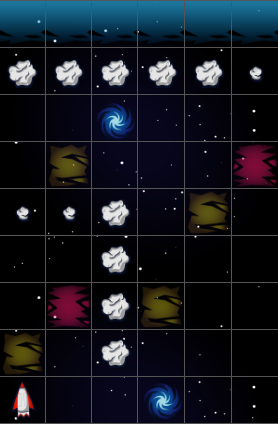
\includegraphics[width=.9\textwidth]{img/spaceworld}
\end{subfigure}
\begin{subfigure}{.36\textwidth}
\centering
{\lstset{numbers=none}
\begin{lstlisting}
|b |b |b |b |b |b |
|kA|kA|kA|kA|kA|kM|
|k |k |kW|k |k |k |
|k |y |k |k |k |r |
|kM|kM|kA|k |y |k |
|k |k |kA|k |k |k |
|k |r |kA|y |k |k |
|y |k |kA|k |k |k |
|kS|k |k |kW|k |k |
\end{lstlisting}}
\end{subfigure}
\end{center}
\caption{Example of Space World with its source code. TODO: Describe letters; consider replacing code listing with a screenshot from task editor with code highlighting}
\label{fig:spaceworld-source}
\end{figure}


\section{RoboCode}

RoboCode is a language based on Python that is used in task sources for solutions.
It is also meant to be used in more advanced levels as the transitional phase
from block-based to text-based programming.
The requirements for the language are following:
\begin{itemize}
\item easy for beginners, understandable without previous knowledge,
\item conciseness (short, but readable programs),
\item matching Blockly blocks closely (for easy transition from Blockly),
\item matching Python closely (for easy transition to Python).
\end{itemize}

\subsection{Syntax and Semantic}
\label{sec:syntax-semantic}

% TODO[consider] note on mixing lexer+parser+some semantic analysis
% (which is partially convenient, partially confusing)

There are four commands for performing actions:
\begin{lstlisting}
fly()
left()
right()
shoot()
\end{lstlisting}
Each action is combined with moving one row forward.
The movement takes place after the action, with the exception of left and right turning actions, where the movement and the action happen simultaneously,
i.e. the spaceship flies diagonally to the left or to the right.
% TODO: Rephrase. Is confusing, because the general statement ("movement takes
% place after the action") is only relevant for shoot(), and all the other
% commands are special cases.

Loops and conditional statements are same as in the Python,
with the notable exception of the repeat loop,
which was simplified to the form matching a corresponding
Blockly block, which is easier to understand by beginners:
% TODO: ass robocode highlighting
\begin{lstlisting}
repeat 4:
    fly()
\end{lstlisting}

Tests inside while-loops and if-statements are limited to the following forms
(again in order to match the respective Blockly blocks):
\begin{lstlisting}
position() [==|!=|>|<|>=|<=] [1..6]
color() [==|!=] ['r'|'g'|'b'|'y'|'k']
<test> [and|or] <test>
\end{lstlisting}
The letters in the color-test have the same meaning as in the space world description,
('r' for red, 'g' for green, etc.)


\subsection{RoboAST}

\begin{table}[h]
\begin{center}
\begin{tabular}{l l l}
\toprule
Name & Form & Usage  \\
\midrule
RoboCode     & textual (Python-like) & sample solutions in task sources  \\
MiniRoboCode & compact string & logging, storing in DB, analysis  \\
RoboBlocks   & Blockly blocks & code editor for students  \\
RoboJS       & textual (JavaScript) & interpretation in browser  \\
RoboAST      & json (AST) & common intermediate representation \\
\bottomrule
\end{tabular}
\end{center}
\caption{Different code representaions used within the system.}
\label{tbl:code-representation}
\end{table}

While Python-like RoboCode is convenient for writing sample solutions,
more comact form would be useful for logging, storing in DB and analysis.
Furthermore, we want a visual blocks presentation of the code for students.
Last but not least, a JavaScript equivalent of the code is needed for
interpreting the code in the browser.
(Table \ref{tbl:code-representation} shows overview of all representations.)

To avoid implementing separate transformations between each pair of these
presentations, we introduced a common intermediate representation,
\emph{RoboAST}, which is a simple Abstract Syntaxt Tree in json.
(REF: figure with example)
For each supported presenation it is enough to implement
its parser returning RoboAST object, and
its generator from RoboAST (REF: diagram).
With one parser and one generator for each presentation,
it is possible to transform presentation A
into presentaion B by parsing A into RoboAST and
then generating B from this RoboAST.
This mechanism also allows for switching between RoboCode and RoboBlocks
anytime during writing a solution in the task editor.
% TODO: mention the disadvantage - not able to use functionality provided by Blockly (code generators)

TODO: fig: example of RoboAst + corresponding RoboCode, MiniRoboCode, RoboJS, RoboBlocks

TODO: diagram of all transformations (ast <-> RoboCode, MiniRoboCode, Blockly, JS)

\subsection{Parsing expression grammar}

For parsing RoboCode into RoboAST, we use a \emph{parsing expression grammar}
(PEG) (REF: PEG grammar).
% TODO: verify the following statement
PEG grammars are basically context-free grammmars with ordered rules
and lookahead expressions (TODO: example).
The specific implementation we used (REF) allows for specifying how should each
parsed subexpression be transformed into a subtree of the final AST
The specyfication can be an arbitrary JavaScript code returning the subtree.
% TODO: check grammar
For illustration, there are some examples of RoboCode parsing rules:

\begin{lstlisting}
CompoundStatement
  = IfStatement
  / WhileStatement
  / RepeatStatement

WhileStatement
  = "while" __ t:Test ":" b:Body
    { return { head: "while", test: t, body: b } }

Test
  = CompoundTest
  / SimpleTest
\end{lstlisting}

The main advantage is that it does not require any lexer and the resulting grammar
is still simple and readable.
The PEG grammar for RoboCode (as described in section \ref{sec:syntax-semantic})
has about 100 lines of code.
However, some preprocessing of the RoboCode is needed, because
PEG is context-free grammar,
while RoboCode is context-sensitive language
-- the context is created by indentation.
In addition, we also want to store line numbers alongside the statements
(useful for meta-interpreting:
showing executed line,
linking errors to the point in source code).
Therefore, the preprocessing step transform the code in the following context-free form,
where each line of code is prepended corresponding line number,
and ``>'' and ``<'' characters denote adding and removing an indentation level, respectively:

\begin{lstlisting}
1| fly()
2| while color() == 'b':
>
3| left()
4| right()
<
5| fly()
\end{lstlisting}

TODO: fig: robocode with corresponding parse tree

\subsection{MiniRoboCode}

\begin{itemize}
\item describe miniRoboCode format - why and what
\end{itemize}

\subsection{RoboBlockly}

\begin{itemize}
\item describe RoboBlockly + images
\end{itemize}


\subsection{RoboJS}

\begin{itemize}
\item describe RoboCodeJS + why
\end{itemize}

\subsection{Interpretation}

\begin{itemize}
\item describe JS interpreter
\item Blockly -> RoboAST -> RoboJS + hooks -> interpreter
\end{itemize}


Example RoboCode, solution of the "Red Shooting" task (currently in figure: \ref{fig:spaceworld-source}), TBA: also include MiniRoboCode, JS, Blockly and AST for complete example.

\begin{lstlisting}
while color() != 'b':
    if color() == 'y':
        right()
    if color() == 'r':
        shoot()
    fly()
\end{lstlisting}

\chapter{Analysis of Collected Data}
\label{chap:analysis}

TBA

\section{Data Description}

TBA, including descriptive statistic and visualization


\section{Explorative Analysis}

TBA


\section{Hypothesis Testing}

TBA


\section{Results}

TBA

\chapter{Conclusion}
\label{chap:conclusion}

\section{Summary}
\label{sec:conclusion.summary}

TBA

\section{Future work}
\label{sec:conclusion.future-work}

TBA


\printbibliography[heading=bibintoc]

\appendix

\chapter{Glossary}
\label{chap:glossary}

\begin{description}
    \item[Flow] TBA: add definition of flow.
\end{description}

\chapter{Data Attachment}
\label{chap:data}

TBA: data attachment

\end{document}
